% TEMPLATE for Usenix papers, specifically to meet requirements of
%  USENIX '05
% originally a template for producing IEEE-format articles using LaTeX.
%   written by Matthew Ward, CS Department, Worcester Polytechnic Institute.
% adapted by David Beazley for his excellent SWIG paper in Proceedings,
%   Tcl 96
% turned into a smartass generic template by De Clarke, with thanks to
%   both the above pioneers
% use at your own risk.  Complaints to /dev/null.
% make it two column with no page numbering, default is 10 point

% Munged by Fred Douglis <douglis@research.att.com> 10/97 to separate
% the .sty file from the LaTeX source template, so that people can
% more easily include the .sty file into an existing document.  Also
% changed to more closely follow the style guidelines as represented
% by the Word sample file. 

% Note that since 2010, USENIX does not require endnotes. If you want
% foot of page notes, don't include the endnotes package in the 
% usepackage command, below.

\documentclass[letterpaper,twocolumn,10pt]{article}
% Preamble
\usepackage{booktabs}
\usepackage{tabularx}
\usepackage{array}
\usepackage{makecell}
\usepackage{usenix,epsfig,endnotes}
\usepackage{amsmath}
\usepackage{booktabs}
\usepackage{makecell}
\usepackage{algorithm}
\usepackage{algpseudocode}
\usepackage{tabularx}
\begin{document}

%don't want date printed
\date{}

%make title bold and 14 pt font (Latex default is non-bold, 16 pt)
\title{\Large \bf RAVEL: Reversible SLO-Aware Virtual Placement for Geo-Distributed LLM Serving}

% \author{
% {\rm Your N.\ Here}\\
% Your Institution
% \and
% {\rm Second Name}\\
% Second Institution
% }

\maketitle

% Use the following at camera-ready time to suppress page numbers.
% Comment it out when you first submit the paper for review.
\thispagestyle{empty}


\subsection*{Abstract}


Geo-distributed LLM serving pools GPU capacity across regions, but WAN
latency and heterogeneous SLOs make the \emph{value} of regional capacity
request-dependent: a region that is optional for one request may be the only
SLO-feasible choice for another. Committing placement immediately preserves
SLO slack but acts on incomplete demand information, whereas waiting to
observe subsequent arrivals consumes the very slack needed to meet the SLO.

We present RAVEL, an SLO-aware serving system that separates when demand
becomes visible from when placement becomes final. RAVEL tentatively assigns
each request to a serving replica and immediately attributes its prospective
demand there, while keeping the assignment revisable until successful engine
handoff. Subsequent arrivals can therefore redirect still-router-owned work
when scarce capacity is needed by more region-constrained requests. Because
reassignment ends at handoff, RAVEL requires no migration of engine-managed
KV state.

We implement RAVEL on vLLM across three geo-distributed clusters connected by
physical WAN paths. Across conversational, bursty, and completion-oriented
workloads, RAVEL improves request-level SLO attainment by XX\%, reduces P95
TTFT by XX\%, and increases SLO-constrained serving capacity by XX\%.




\begin{figure}[t]
    \centering
    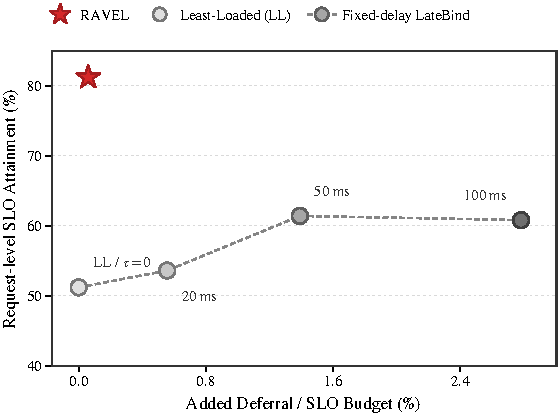
\includegraphics[width=\columnwidth]{motivation.pdf}
    \caption{
    \textbf{Information--slack tradeoff.}
    Fixed-delay late binding consumes SLO slack to observe more demand;
    RAVEL accounts demand immediately and selectively uses a
    request-specific, slack-bounded mobility hold for pre-handoff replanning.
    }
    \label{fig:motivation}
\end{figure}


\section{Introduction}
\label{sec:introduction}

LLM serving is increasingly expanding beyond scheduling replicas within a
single cluster toward pooling inference capacity across geographically
distributed clusters~\cite{skylb,gorgo,solyx}.
Geo-distribution gives a service more capacity choices, but also makes the
choice of serving site consequential: a placement determines not only GPU load
and cache locality, but also the WAN path and remote serving conditions a
request encounters.
At the same time, serving traffic has become increasingly heterogeneous.
Interactive requests may impose tight time-to-first-token (TTFT) and
time-between-token (TBT) bounds, whereas longer-running or multi-stage
requests may instead be governed by end-to-end completion deadlines
~\cite{distserve,jitserve}.
The combination of geographic and SLO heterogeneity means that available GPU
capacity is not equally useful to every request.

Existing distributed and geo-distributed routers therefore make increasingly
informed placement decisions, incorporating load, network latency, cache
locality, and request-level SLOs when choosing where an arrival should
execute~\cite{preble,dualmap,skylb,gorgo,quartz}.
These mechanisms improve the destination selected for the request and system
state visible \emph{now}.
We find, however, that heterogeneous SLOs create an additional online
allocation problem: a placement that is locally attractive for the current
request can consume regional capacity that a later request may be unable to
replace.
The relevant question is therefore not only
\emph{where should this request execute?}, but also
\emph{when should an earlier placement become final?}

Consider two serving regions, $A$ and $B$, and two requests, $r_1$ and $r_2$.
Let $\mathcal{F}_i$ denote the set of regions in which request $i$ can satisfy
its SLO.
Suppose
$\mathcal{F}_1=\{A,B\}$, while
$\mathcal{F}_2=\{A\}$.
When $r_1$ arrives first, $A$ may be its faster destination, making an
assignment to $A$ locally preferable.
Doing so, however, can consume the only SLO-feasible capacity available to
$r_2$ when it arrives shortly afterward; assigning $r_1$ to $B$ instead can
allow both requests to succeed.
\emph{Region $A$ is merely faster for $r_1$, but it is essential for $r_2$.}
Thus, the \emph{value} of regional capacity is request-dependent:
capacity that is interchangeable for a flexible request may be indispensable
to a more region-constrained one.
Consequently, optimizing each placement independently need not maximize
request-level SLO attainment.

The difficulty is temporal rather than merely predictive.
When $r_1$ arrives, even an accurate router can estimate only the demand and
serving state visible at that time; it cannot know whether a more constrained
request such as $r_2$ will arrive next.
Making the placement final immediately preserves SLO slack, but can lock in an
allocation before this information becomes available.
A natural alternative is to wait for subsequent arrivals before deciding,
as in delayed-scheduling and late-binding approaches
~\cite{delayscheduling,sparrow}.
For SLO-constrained inference, however, this information is not free:
every millisecond spent waiting also consumes the same SLO budget needed for
WAN transfer, queueing, and inference.
We refer to this tension as the
\emph{information--slack tradeoff}.
Figure~\ref{fig:motivation} makes the tradeoff visible empirically.
Fixed-delay late binding can improve SLO attainment when a short wait exposes
useful arrivals, but increasing the delay eventually erodes those gains as
more SLO slack is consumed.

RAVEL is built around a simple observation:
\emph{waiting to finalize placement need not mean waiting to account for
demand}.
Rather than treating placement as a single atomic decision, RAVEL separates
when an arrival becomes visible to capacity planning from when its destination
becomes final.
On arrival, RAVEL tentatively assigns the request to a serving replica and
immediately attributes its prospective demand to that replica.
Later requests therefore observe the demand of earlier arrivals even while
those earlier placements remain revisable.
When additional observation is useful, RAVEL can selectively keep eligible
non-LATENCY requests router-owned for a short, request-specific mobility hold
bounded by both remote RTT and predicted SLO slack.
Unlike fixed-delay late binding, these requests are already placed and
accounted during the hold.
New arrivals may then trigger bounded replanning of still-router-owned
requests.
A placement becomes final only after successful engine handoff; because RAVEL
stops reassignment at this boundary, it never needs to migrate
engine-managed KV state.

Realizing this abstraction requires addressing three systems challenges.
First, RAVEL must determine which replicas remain SLO-feasible for each
request under heterogeneous WAN delays, engine backlog, Prefill and Decode
interference, and request-specific success criteria.
RAVEL addresses this using calibrated, replica-specific SLO quotes derived
from live serving state.
Second, tentative work must influence subsequent decisions without becoming
double-counted or stale when its placement changes.
RAVEL therefore maintains prospective accounting whose queue ownership and
replica-dependent charges move with a reassignment.
Third, retaining revisability cannot require repeatedly optimizing over all
outstanding requests or allowing a deep engine queue to hide work from the
router.
RAVEL limits expensive replanning to a bounded router-owned cohort and keeps
the engine-visible frontier shallow, while SLO-specific admission and local
Prefill control preserve latency-sensitive execution constraints.

We implement RAVEL as an asynchronous routing layer for
vLLM~\cite{vllm} and evaluate it on five serving replicas across three
clusters connected by physical WAN paths.
Our experiments cover conversational traffic, bursty arrivals, and
completion-oriented demand over six offered-load levels.
At $16\times$ load, RAVEL improves request-level SLO attainment over the
best-SLO baseline by \textbf{8.8}, \textbf{17.2}, and
\textbf{16.6 percentage points} on LMSYS, Burst, and DeepResearch,
respectively.
Across the same three workloads, it reduces P95 TTFT by
\textbf{21.8--69.2\%} relative to the corresponding best-SLO baseline.
On Burst, for example, RAVEL increases SLO attainment from 62.0\% to 79.2\%
while reducing P95 TTFT from 8.70\,s to 2.68\,s and P95 end-to-end latency
from 28.68\,s to 18.78\,s.
Its online replanning path remains millisecond-scale, with a measured P95
scheduling-pass latency of 2.10\,ms at Burst $12\times$ load.

In summary, this paper makes three contributions:
\begin{itemize}
    \item
    We identify the \emph{request-dependent value of regional capacity} in
    geo-distributed LLM serving: heterogeneous SLOs make capacity
    interchangeable for some requests but essential for others, so optimizing
    placements independently can reduce aggregate request-level SLO
    attainment.

    \item
    We introduce an \emph{immediate-accounting, deferred-commitment}
    abstraction that makes arrived demand visible immediately while retaining
    pre-handoff placement revisability.
    RAVEL realizes this abstraction through replica-specific SLO quotes,
    transferable prospective accounting, slack-bounded mobility, and bounded
    cohort replanning.

    \item
    We implement RAVEL on vLLM and evaluate it on a physical-WAN deployment,
    showing substantial SLO-attainment gains across heterogeneous,
    bursty, and completion-oriented workloads while keeping online replanning
    at millisecond-scale latency.
\end{itemize}

\section{Problem and Design Opportunity}
\label{sec:problem}

We distinguish three concepts that are often coupled in request routing:
\emph{placement}, \emph{regional demand accounting}, and
\emph{commitment}.
A placement is the serving region currently associated with a request.
Regional demand accounting attributes an arrived request's prospective work
to a region so that the request influences subsequent placement decisions.
Commitment, by contrast, is the point after which RAVEL no longer revises
that placement.
RAVEL chooses successful handoff to the serving engine as this boundary:
requests remain reassignable while they are router-owned, whereas their
placement becomes final after handoff.
This is a deliberate control-plane boundary rather than an inherent
irreversibility property of LLM execution; it lets RAVEL revise placement
without coordinating migration of engine-managed request state.


\subsection{Request-Dependent Regional Feasibility}
\label{sec:problem:feasibility}

Geo-distributed serving exposes each request to different WAN and serving
conditions depending on its destination.
At the same time, requests differ in the SLO constraints they must satisfy.
For request $i$ and serving region $c$, let
$\Phi_{i,c}(t)$ indicate whether, using information available at time $t$,
region $c$ is predicted to satisfy all SLO constraints applicable to $i$.
This prediction depends on the request's SLO semantics and remaining slack,
its estimated service demand, the WAN path to $c$, and the currently observed
serving conditions at that region.
Section~\ref{sec:design:feasibility} describes how RAVEL constructs these
predictions at replica granularity.

We define the feasible-region set of request $i$ as
\begin{equation}
    \mathcal{F}_i(t)
    =
    \left\{
        c \mid \Phi_{i,c}(t)=1
    \right\}.
    \label{eq:problem:feasible-set}
\end{equation}
The time dependence is important.
Even if network and serving conditions remain unchanged,
$\mathcal{F}_i(t)$ may shrink while a request waits because the waiting time
itself consumes remaining SLO slack.

Feasible sets characterize how substitutable regional capacity is for a
request.
A request with many feasible regions has several serving alternatives,
whereas a request with a small feasible set may depend on capacity in only one
or two regions.
Consequently, assigning scarce SLO-feasible capacity to broadly feasible work
can remove the only viable option for more region-constrained requests.
Regional capacity is therefore not equally substitutable across requests, and
optimizing request--region assignments independently need not maximize
aggregate request-level SLO attainment.


\subsection{The Information--Slack Tradeoff}
\label{sec:problem:tradeoff}

The difficulty is that this scarcity is revealed online.
When a request arrives, the router observes only the requests and system state
available at that time.
Subsequent arrivals may reveal that capacity tentatively allocated earlier is
more valuable to newly arrived, region-constrained requests.
Thus, the desirable allocation can change while earlier requests are still
waiting to execute.

Table~\ref{tab:problem:operating-points} separates three operating points by
when arrived demand becomes visible to regional planning and when placement
becomes final.
A conventional one-shot router assigns an arriving request immediately:
its demand is attributed to a region at once, but the placement is not revised
after that routing decision.
At the other extreme, our diagnostic LateBind-$\tau$ policy keeps a request
centrally unassigned for $\tau$, then observes the current state and makes a
single placement decision.
LateBind-$\tau$ therefore postpones both regional demand attribution and
placement commitment.
RAVEL targets the remaining operating point: it attributes demand
immediately, while keeping the tentative placement revisable until engine
handoff.



\begin{table}[t]
    \centering
    \small
    \caption{Accounting and placement-finality operating points.}
    \label{tab:problem:operating-points}

    \renewcommand{\arraystretch}{1.25}

    \begin{tabular*}{\columnwidth}{
        @{\extracolsep{\fill}}
        lcc
        @{}
    }
        \toprule
        \textbf{Policy} &
        \textbf{Demand accounting} &
        \textbf{Placement finality} \\
        \midrule
        One-shot        & Immediate & Immediate \\
        LateBind-$\tau$ & Deferred  & Deferred  \\
        RAVEL           & Immediate & Deferred  \\
        \bottomrule
    \end{tabular*}
\end{table}

Deferring a decision can expose useful information, but that information has a
direct cost under request SLOs.
Holding request $i$ for $\tau$ consumes $\tau$ of the same budget needed for
WAN transfer, queueing, and inference.
A longer delay may therefore expose more subsequent demand while
simultaneously reducing the set of regions in which the held request can still
succeed.
Equivalently, $\mathcal{F}_i(t)$ can shrink purely because the router waits,
even without any increase in serving load.
We refer to this tension as the
\emph{information--slack tradeoff}.
Figure~\ref{fig:motivation} illustrates it empirically:
short fixed deferral can sometimes improve placement, whereas additional
waiting eventually erodes SLO attainment.

The resulting design opportunity is to separate
\emph{when an arrived request begins influencing regional capacity planning}
from
\emph{when its placement becomes final}.
Doing so requires three capabilities:
RAVEL must determine request-specific SLO feasibility,
transfer prospective demand accounting when a tentative placement changes,
and bound both deliberate holding and multi-request replanning so that the
control mechanism does not itself consume excessive SLO slack.
Section~\ref{sec:design} describes how RAVEL realizes these requirements.



\begin{figure*}[t]
    \centering
    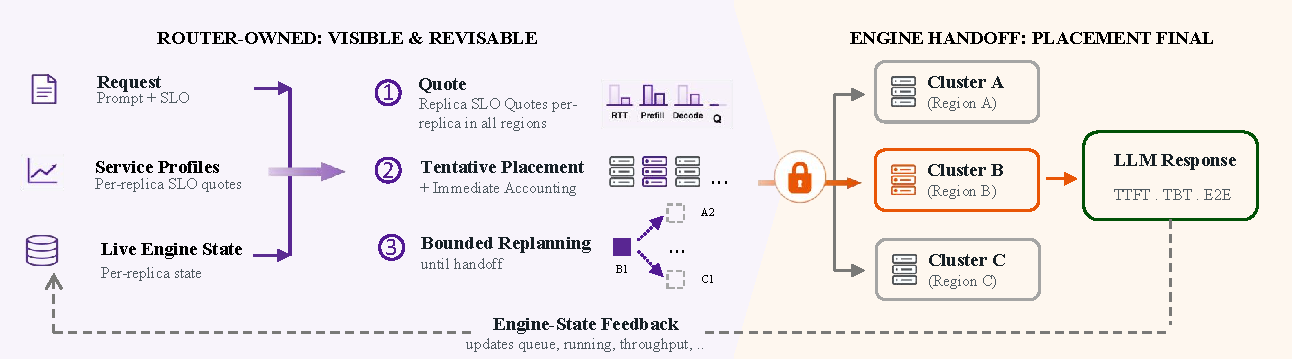
\includegraphics[
        width=\textwidth
    ]{RAVEL_System_cropped.pdf}
    \caption{
    \textbf{RAVEL system overview.}
    During the router-owned phase, RAVEL constructs replica-specific SLO
    quotes from the request, calibrated service profiles, and live engine
    state; it then selects a tentative replica, immediately accounts the
    request's prospective demand, and may revise the placement through bounded
    replanning.
    A successful engine-facing posting-task handoff makes the selected
    placement final.
    The serving engine subsequently executes the request, while observed
    engine state feeds back into later routing decisions.
    Purple denotes router-owned and revisable state; orange denotes handoff
    and committed placement.
    }
    \label{fig:ravel-overview}
\end{figure*}



\section{RAVEL Design}
\label{sec:design}
\subsection{overview}
\label{sec:design:overview}

RAVEL is a geo-routing control layer that separates
\emph{regional demand accounting} from \emph{placement commitment}.
As shown in Figure~\ref{fig:ravel-overview}, RAVEL sits between clients and
the serving engines deployed across regions.
While a request remains router-owned, RAVEL maintains a tentative regional
placement that may still be revised.
Handoff to the selected serving engine is RAVEL's commitment boundary; after
handoff, the regional placement is fixed and the backend proceeds with normal
LLM execution, e.g., using vLLM~\cite{vllm}.

RAVEL bases placement on request-specific SLOs and service-demand estimates,
network conditions, and regional load.
Crucially, its load view combines \emph{observed engine-owned work} with
\emph{prospective router-owned work}: the former reflects work already handed
to serving engines, whereas the latter represents arrived demand whose
regional placement remains revisable.
When a request $i$ arrives, RAVEL determines its currently SLO-feasible
regions, selects a tentative placement, and immediately attributes $i$'s
prospective work to the selected region.
The tentative placement therefore affects subsequent routing decisions
immediately even though it has not yet been committed.

When RAVEL replans an eligible, bounded set of uncommitted requests, it may
revise their tentative regional placements.
Across its SLO-specific planners, RAVEL prioritizes allocations predicted to
preserve request SLOs; among viable alternatives, it uses prospective regional
load and calibrated service demand to guide placement.
When a request moves from region $A$ to region $B$, its prospective demand
accounting moves with it: the charge to $A$ is removed and the corresponding
charge is attributed to $B$.
Thus, each tentatively placed router-owned request is logically accounted to
\emph{exactly one region at a time}, even if its placement changes.

At engine handoff, the tentative placement becomes final and the serving
engine executes the request normally.
Engine-load and request-lifecycle updates feed back into RAVEL's online state
and inform subsequent decisions.
The remainder of this section describes how RAVEL estimates request-specific
regional feasibility, maintains prospective demand accounting, performs
bounded pre-admission reassignment, and coordinates engine handoff.



\subsection{Replica SLO Quotes}
\label{sec:design:feasibility}

RAVEL separates estimating a request--replica assignment from choosing that
assignment.
Let $c \in \mathcal{C}$ denote a geographic serving cluster,
$\mathcal{R}_c$ its replicas, and $c(r)$ the cluster containing replica $r$.
For each request $i$ and candidate replica $r$, RAVEL constructs a
\emph{replica quote} from the currently observed system state.
The enclosing cluster $c(r)$ determines WAN latency and calibrated service
curves, while queue and engine state are replica-specific.
A quote predicts the SLO-relevant cost of assigning $i$ to $r$ and whether
that assignment is currently feasible; later sections decide how these quotes
are used for accounting and placement.

\paragraph{Calibrated service model.}
RAVEL profiles each serving configuration rather than assuming a fixed
token-processing rate.
At active-Decode concurrency $n$, it uses an affine planning model for the
Prefill-side first-token service component,
\begin{equation}
    P_{c,n}(p) = b_{c,n} + a_{c,n}p,
    \label{eq:ravel-prefill-profile}
\end{equation}
where $p$ is the prompt length, $a_{c,n}$ is the profiled seconds per prompt
token, and $b_{c,n}$ captures fixed Prefill overhead.
For Decode, RAVEL uses the calibrated median post-first-token TPOT,
$d_c(n)$, at each measured concurrency level.
At runtime it interpolates between measured points and clips outside the
profiled range.
Because the Prefill curves are measured under the corresponding Decode
concurrency, RAVEL does not add a separate Decode-interference penalty to its
TTFT estimate.

\paragraph{TTFT and Decode estimates.}
Let $p_i$ be request $i$'s prompt length.
Because the router's shadow prefix state does not certify actual engine cache
residency, RAVEL charges the full prompt for feasibility estimation and uses
estimated prefix hits only as a secondary locality signal.

For replica $r$, let $W_r^{\mathrm{eng}}$ be its outstanding engine-side
Prefill work in prompt tokens and $Q_r^{\mathrm{eng}}$ its pending-request
count.
Let $W_{i,r}^{\mathrm{ahead}}$ and $Q_{i,r}^{\mathrm{ahead}}$ denote
router-owned work ordered no later than $i$ under RAVEL's absolute-SLO-deadline
order,
\[
    (a_i + D_i,\; a_i,\; id_i),
\]
including earlier tentative assignments made in the current planning pass.
With $n_r$ currently running sequences, RAVEL estimates
\begin{align}
\widehat{S}^{\mathrm{pre}}_{i,r}
&=
\left(
W_r^{\mathrm{eng}}
+ W_{i,r}^{\mathrm{ahead}}
+ p_i
\right)a_{c(r),n_r}
\nonumber\\
&\quad+
\left(
Q_r^{\mathrm{eng}}
+ Q_{i,r}^{\mathrm{ahead}}
+ 1
\right)b_{c(r),n_r},
\label{eq:ravel-prefill-quote}\\
\widehat{\mathrm{TTFT}}_{i,r}(t)
&=
(t-a_i)
+
\rho_{o_i,c(r)}
+
\widehat{S}^{\mathrm{pre}}_{i,r},
\label{eq:ravel-ttft}
\end{align}
where $\rho_{o_i,c(r)}$ is the RTT from request origin $o_i$ to cluster
$c(r)$.
Including elapsed time makes feasibility explicitly slack-dependent: a
replica may become infeasible while a request waits even if network and
serving state remain otherwise unchanged.

For Decode, RAVEL uses a conservative prospective sequence count $m_{i,r}$
that includes outstanding router-owned, engine-pending, and running requests
associated with $r$, counting each request logically once.
This quantity is a planning proxy rather than an exact prediction of which
sequences will overlap.
The predicted per-token Decode time is then $d_{c(r)}(m_{i,r})$.

\paragraph{Latency-sensitive SLOs.}
For a latency-sensitive request with TTFT and TBT bounds
$D_i^{\mathrm{TTFT}}$ and $D_i^{\mathrm{TBT}}$, replica $r$ is feasible iff
\begin{equation}
\Phi^{\mathrm{lat}}_{i,r}(t)
=
\mathbf{1}\!\left[
\widehat{\mathrm{TTFT}}_{i,r}(t)
\le D_i^{\mathrm{TTFT}}
\;\land\;
d_{c(r)}(m_{i,r})
\le D_i^{\mathrm{TBT}}
\right].
\label{eq:ravel-latency-feasible}
\end{equation}
RAVEL therefore retains TTFT and TBT as separate feasibility constraints.
For later placement decisions, it additionally maps TBT pressure onto the
TTFT scale,
\begin{equation}
\widehat{T}^{\mathrm{lat,obj}}_{i,r}
=
\max\!\left\{
\widehat{\mathrm{TTFT}}_{i,r},
\;
D_i^{\mathrm{TTFT}}
\frac{d_{c(r)}(m_{i,r})}{D_i^{\mathrm{TBT}}}
\right\}.
\label{eq:ravel-latency-objective}
\end{equation}
This scalar is an \emph{ordering signal}, not a replacement for
Equation~\ref{eq:ravel-latency-feasible}: feasibility still requires both
TTFT and TBT constraints to hold individually.

\paragraph{Completion-oriented SLOs.}
For completion requests, RAVEL distinguishes an expected output demand
$L_i^{\mathrm{exp}}$ from a conservative risk demand
$L_i^{\mathrm{risk}}$:
\begin{align}
\widehat{T}^{\mathrm{point}}_{i,r}
&=
\widehat{\mathrm{TTFT}}_{i,r}
+
(L_i^{\mathrm{exp}}-1)d_{c(r)}(m_{i,r}),
\nonumber\\
\widehat{T}^{\mathrm{risk}}_{i,r}
&=
\widehat{\mathrm{TTFT}}_{i,r}
+
(L_i^{\mathrm{risk}}-1)d_{c(r)}(m_{i,r}).
\label{eq:ravel-completion-objectives}
\end{align}
Outside the completion-specific soft-admission regime, feasibility uses the
risk estimate,
\begin{equation}
\Phi^{\mathrm{comp}}_{i,r}(t)
=
\mathbf{1}\!\left[
\widehat{T}^{\mathrm{risk}}_{i,r}(t)
\le D_i^{\mathrm{comp}}
\right].
\label{eq:ravel-completion-feasible}
\end{equation}
These output demands are derived from request-visible information rather than
realized generation length.
When the soft-admission epoch is active and a semantic expected-output
estimate is available, RAVEL instead uses that expected estimate for both
point and risk demand in its on-time-set planning; Section~\ref{sec:design:policy}
describes this completion-specific policy.

A replica quote therefore carries the point- and risk-oriented latency
estimates needed by the request's SLO semantics, the Prefill-side
queue/service estimate in Equation~\ref{eq:ravel-prefill-quote}, and the
resulting feasibility decision.
This Prefill-side estimate should not be confused with the
\emph{own-service virtual demand} introduced next, which RAVEL uses for
prospective regional demand accounting.


\subsection{Prospective Regional Demand Accounting}
\label{sec:design:accounting}

Replica quotes characterize the consequence of a placement, but later
decisions must also observe demand from requests that have arrived without yet
committing to an engine.
RAVEL makes such demand visible immediately through two complementary
mechanisms.
\emph{Queue-based prospective accounting} captures the direct Prefill
queueing externality of router-owned requests, while
\emph{virtual placement accounting} captures target-dependent service and
latency-admission externalities that queue position alone does not express.
RAVEL realizes regional demand accounting at replica granularity, since a
region may contain multiple independently loaded replicas.
Importantly, demand attribution does not imply commitment: while a request
remains router-owned, both its tentative replica owner and the accounting
associated with that owner may still change.

\paragraph{Queue-based prospective accounting.}
When request $i$ is tentatively assigned to replica $r$, RAVEL places it in
$r$'s router-owned queue.
Its full prompt work $p_i$ is therefore immediately visible to later replica
quotes.
Under the absolute planning-deadline order $\kappa$, requests ordered no later
than a quoted request $j$ contribute to
$W^{\mathrm{ahead}}_{j,r}$.
Within a replanning pass, RAVEL similarly incorporates the prompt work and
request count of each earlier tentative assignment into the pass-local state
seen by subsequent candidates.
Thus, an arrived request can affect later placement decisions before either
request has crossed the engine-handoff boundary.
RAVEL requires no separate \emph{persistent} aggregate prompt-work ledger:
tentative queue ownership and pass-local planning state together provide
prospective Prefill accounting. 

\begin{table}[t]
\centering
\small
\caption{Prospective planning signals used by RAVEL.}
\label{tab:ravel-demand-state}
\begin{tabular}{@{}llll@{}}
\toprule
Signal
& \makecell{Per-request\\quantity}
& \makecell{Derived /\\aggregate state}
& Role \\
\midrule
Prefill
& $p_i$
& $W^{\mathrm{ahead}}_{i,r}$
& Prefill queueing \\
Service
& $s^{\mathrm{own}}_{i,r}$
& $L_r$
& Service balance \\
TBT
& $u_{i,r}$
& $A_r$
& TBT admission balance \\
\bottomrule
\end{tabular}
\end{table}

\paragraph{Virtual service accounting.}
Prompt tokens alone do not capture heterogeneous service cost: the same
request can consume different service time at different replicas.
RAVEL therefore assigns request $i$ a replica-dependent own-service charge.
Its own Prefill component is
\begin{equation}
s^{\mathrm{pre,own}}_{i,r}
=
b_{c(r),n_r}
+
a_{c(r),n_r}p_i ,
\label{eq:ravel-own-prefill}
\end{equation}
while its own Decode component is
\begin{equation}
s^{\mathrm{dec,own}}_{i,r}
=
\begin{cases}
(L_i^{\mathrm{exp}}-1)d_{c(r)}(m_{i,r}),
    & \text{completion-oriented},\\
0,
    & \text{LATENCY}.
\end{cases}
\label{eq:ravel-own-decode}
\end{equation}
RAVEL then defines
\begin{equation}
s^{\mathrm{own}}_{i,r}
=
s^{\mathrm{pre,own}}_{i,r}
+
s^{\mathrm{dec,own}}_{i,r}.
\label{eq:ravel-own-service}
\end{equation}
This matches RAVEL's point estimate: completion requests contribute their
expected Decode service, whereas LATENCY requests express Decode pressure
through the TBT-specific signal below. 

The own-service charge is distinct from the queue-inclusive
$\widehat{S}^{\mathrm{pre}}_{i,r}$ in
Equation~\ref{eq:ravel-prefill-quote}.
The latter includes engine-side backlog and queue-ahead work to predict
Prefill-side delay; $s^{\mathrm{own}}_{i,r}$ captures only the
replica-dependent service demand induced by request $i$ itself.

RAVEL accumulates these charges in $L_r$, an
\emph{active-request virtual service load}.
A request contributes its profiled charge when it is assigned, the charge is
transferred if its owner changes, and it is released when the request
terminates.
$L_r$ therefore tracks profiled charges of active requests rather than their
instantaneous remaining service.
It complements engine telemetry: observed pending and running work describes
current execution state, whereas $L_r$ immediately reflects the service
consequences of RAVEL's own placement decisions. 

\paragraph{Latency-admission accounting.}
Service time alone does not capture how strongly a LATENCY request constrains
Decode relative to its TBT requirement.
RAVEL therefore defines
\begin{equation}
u_{i,r}
=
\frac{d_{c(r)}(1)}
     {D_i^{\mathrm{TBT}}},
\label{eq:ravel-tbt-demand}
\end{equation}
where $d_{c(r)}(1)$ is the calibrated single-sequence Decode TPOT.
The ratio is dimensionless and represents the fraction of one allowed TBT
period consumed by the replica's single-sequence token service time.
RAVEL accumulates these charges in a latency-admission ledger $A_r$.


$A_r$ serves a different purpose and has a different lifetime from $L_r$.
It is an admission-side balancing signal rather than an estimate of
outstanding Decode work.
In particular, $A_r$ should not be confused with the prospective sequence
count $m_{i,r}$: the latter estimates Decode concurrency for request-level
feasibility, whereas $A_r$ records how much TBT-normalized demand RAVEL has
assigned to a replica.
Unlike $L_r$, $A_r$ is cumulative within a scheduler run:
reassignment transfers a LATENCY request's charge to its new owner, but
request completion does not decrement the ledger.
The placement policy consults $A_r$ only after request-level feasibility and
lateness have been considered. 


\paragraph{Accounting follows reassignment.}
Let $x_i$ denote the current tentative replica owner of request $i$.
If replanning changes $x_i$ from replica $r$ to replica $r'$, RAVEL transfers
the request's queue ownership and replaces each applicable virtual charge with
the target-specific charge of $r'$:

\begin{align}
L_r      &\gets L_r      - s^{\mathrm{own}}_{i,r},
&
L_{r'}   &\gets L_{r'}   + s^{\mathrm{own}}_{i,r'}, \nonumber\\
A_r      &\gets A_r      - u_{i,r},
&
A_{r'}   &\gets A_{r'}   + u_{i,r'}.
\label{eq:ravel-accounting-transfer}
\end{align}

The new charges are recomputed rather than copied because service
characteristics may differ across target replicas. 

While router-owned, each request belongs to exactly one replica queue, so its
prompt work is represented once.
Each virtual accounting mechanism likewise associates a registered charge
with at most one replica at a time; reassignment replaces the old charge with
the target-specific charge.
Service charges remain active through engine handoff and are released at
request termination, whereas latency-admission charges persist as cumulative
admission state within the scheduler run.
Together, these mechanisms make the consequences of an assignment visible
before that assignment becomes irrevocable.
Section~\ref{sec:design:replanning} next describes when RAVEL may reconsider
these tentative assignments.


\subsection{Bounded Replanning}
\label{sec:design:replanning}

Immediate accounting makes tentative placements visible to subsequent
decisions, but RAVEL does not continuously reconsider every outstanding
request.
Instead, it replans a selected cohort whose placements remain under router
control.
Requests that have crossed the engine-handoff boundary are no longer eligible
for router-level reassignment, although their pending and running work
continues to affect replica quotes.
RAVEL therefore separates the \emph{reversible set} that may be reassigned
from the larger set of requests that still influence placement decisions.

\paragraph{Replanning triggers.}
Every arriving request first receives a tentative placement and the
corresponding accounting from Sections~\ref{sec:design:feasibility} and
\ref{sec:design:accounting}.
A LATENCY arrival triggers cohort replanning immediately; the arriving request
itself enters the mobile cohort only if a remote cluster contains a currently
SLO-feasible replica.
A non-LATENCY arrival also triggers replanning when it receives no mobility
hold.
Otherwise, RAVEL arms a timer for the hold expiration and invokes replanning
when that timer fires.
Completion events that release active-request virtual service load $L_r$
likewise request replanning.
When the completion-specific soft-admission regime is active, scheduler
invocations also replan the current completion cohort before admission.

\paragraph{Slack-bounded mobility hold.}
For selected non-LATENCY requests, RAVEL deliberately prevents immediate
engine dispatch for a short \emph{mobility hold}.
The hold is computed once when the request arrives.
Let
\begin{equation}
\sigma_i^{\mathrm{arr}}
=
\max\!\left\{
0,\;
\Delta_i -
\min_r \widehat{T}^{\mathrm{obj}}_{i,r}(a_i)
\right\}
\label{eq:ravel-arrival-slack}
\end{equation}
denote the predicted placement slack at arrival, and let
$\rho_i^{\min}$ be the minimum positive RTT from $i$'s origin to a remote
serving cluster.
RAVEL identifies a burst when the most recent inter-arrival gap falls within
the observed cross-region decision horizon; in the implementation, this means
that the gap does not exceed the largest RTT to a remote cluster.
If such a burst is observed and at least two serving clusters contain an
SLO-feasible replica, RAVEL sets
\begin{equation}
h_i
=
\min\!\left\{
\rho_i^{\min},
\sigma_i^{\mathrm{arr}}
\right\};
\label{eq:ravel-mobility-hold}
\end{equation}
otherwise $h_i=0$.
LATENCY requests always use $h_i=0$.

The mobility hold is not the full duration for which a placement remains
reversible.
While $h_i$ is active, request $i$ remains router-owned and is ineligible for
engine dispatch, while its tentative placement and accounting may still be
revised.
Expiration of $h_i$ merely makes $i$ eligible for dispatch; if engine capacity
or admission conditions prevent handoff, the request remains in the router
queue and can continue to participate in later replanning.
Thus, the hold consumes at most a bounded portion of predicted slack, while
demand accounting begins immediately at arrival.

\paragraph{Bounded candidate cohort.}
At each replanning event, RAVEL collects requests from the router-owned queues
across replicas.
For a LATENCY request, mobility eligibility additionally requires at least one
SLO-feasible replica in a remote cluster.
RAVEL orders eligible requests by $\kappa_i$ and passes only a bounded prefix
to the SLO-specific placement policy.

Let $K$ denote the normal cohort bound.
Under the normal path, at most $K$ requests are passed to one cohort placement
pass.
During completion-specific soft admission, RAVEL may enlarge this bound to
the deployment's total sequence capacity so that the protected completion set
can be considered together.
This bounds the expensive multi-request placement computation, although
candidate discovery itself may inspect the current router queues.

Requests outside the selected cohort retain their current owners and are not
reassigned in that pass.
The SLO-specific policy incorporates applicable non-candidate work as fixed
planning context; Section~\ref{sec:design:policy} describes the completion
policy's special treatment of deferred work.
Within the selected cohort, candidates are processed in planning-deadline
order, and assignments made for earlier candidates update pass-local prompt
work, request counts, and prospective state before later candidates are
quoted.

\paragraph{Applying a replanning result.}
For each candidate $i$, the SLO-specific policy returns a target replica
$x'_i$ together with the quote associated with that assignment.
If $x'_i$ differs from the current tentative owner $x_i$, RAVEL transfers
$i$'s router-queue ownership to $x'_i$.
It then refreshes the applicable target-dependent virtual accounting using
the final assignment and quote.
Accounting refresh is conceptually distinct from ownership transfer:
even when $x'_i=x_i$, a newly constructed quote may change the
replica-dependent service charge associated with the request.

Replanning therefore modifies only tentative router-level placement and
planning state; it does not itself commit a request to an engine.
By restricting the expensive placement pass to a finite router-owned cohort,
RAVEL controls replanning overhead while retaining engine-owned and
non-candidate work as policy-appropriate context.
Section~\ref{sec:design:policy} next specifies how RAVEL chooses placements
within this cohort under different SLO semantics.


\subsection{SLO-Specific Placement and Admission}
\label{sec:design:policy}

Section~\ref{sec:design:replanning} determines when and over which
router-owned requests RAVEL replans.
RAVEL then chooses tentative replicas and controls engine admission according
to the SLO semantics of the observed traffic.
The released policy has two paths.
Once a non-workflow request is observed, RAVEL uses a mixed-traffic path that
preserves TTFT/TBT obligations while accommodating completion-oriented work.
A pure multi-stage completion stream instead uses a completion-oriented path.
Both paths share the replica quotes, prospective accounting, and bounded
replanning mechanisms developed above; they differ only in how they allocate
scarce serving capacity and decide which work may cross the router--engine
frontier.

\paragraph{Mixed TTFT/TBT placement.}
RAVEL processes the selected cohort in planning-deadline order $\kappa_i$.
For request $i$ and legal target replica $r$, define normalized objective
lateness as
\begin{equation}
\ell^{\mathrm{obj}}_{i,r}
=
\frac{
\max\!\left\{
0,\,
\widehat{T}^{\mathrm{obj}}_{i,r}-\Delta_i
\right\}
}{
\Delta_i
},
\label{eq:ravel-objective-lateness}
\end{equation}
and normalized TTFT pressure as
\begin{equation}
\ell^{\mathrm{ttft}}_{i,r}
=
\frac{
\max\!\left\{
0,\,
\widehat{\mathrm{TTFT}}_{i,r}
-
D_i^{\mathrm{TTFT}}
\right\}
}{
D_i^{\mathrm{TTFT}}
}.
\label{eq:ravel-ttft-lateness}
\end{equation}
For LATENCY requests, TTFT is part of the request-level success condition.
For non-LATENCY requests, $D_i^{\mathrm{TTFT}}$ instead provides a
request-visible reference for limiting first-token delay; their success
criterion remains the completion objective.

Let $O_{i,r}$ denote the pending-capacity overflow cost associated with
placing $i$ at $r$.
This term is hold-aware.
LATENCY requests expose pending-capacity overflow immediately, whereas a
non-LATENCY request does not pay this penalty while its mobility hold
deliberately keeps it in the reversible router tier.

RAVEL also discourages concentrating profiled service on a replica.
Let $V^{\mathrm{ctx}}_{i,r}$ denote the queue-inclusive profiled service state
visible immediately before placing $i$ in the current cohort pass.
It reflects engine-side prompt debt, applicable fixed router work, and service
assigned to candidates processed earlier in the pass.
RAVEL defines the convex marginal-service cost
\begin{equation}
M_{i,r}
=
\frac{
\left(
V^{\mathrm{ctx}}_{i,r}
+
s^{\mathrm{own}}_{i,r}
\right)^2
-
\left(
V^{\mathrm{ctx}}_{i,r}
\right)^2
}{
\Delta_i^2
}.
\label{eq:ravel-marginal-work}
\end{equation}
$V^{\mathrm{ctx}}_{i,r}$ is distinct from the virtual service ledger $L_r$
of Section~\ref{sec:design:accounting}.
The former captures queue-inclusive congestion in the current planning
context; the latter carries active-request virtual service load across
placement decisions.
The two signals therefore describe different externalities rather than
double-counting the same state.

Before replanning a cohort, RAVEL removes the candidates' old virtual charges
from the fixed accounting base.
Selections made earlier in $\kappa_i$ order are then added back to pass-local
state before later candidates are considered.
Let $A^{\mathrm{pass}}_{i,r}$ and $L^{\mathrm{pass}}_{i,r}$ denote these
pass-local values immediately before placing $i$, and define
\[
\chi^{\mathrm{lat}}
=
\mathbf{1}[\text{a LATENCY request has been observed}].
\]
The latency-admission and service virtual-finish terms are
\begin{equation}
\widetilde{A}_{i,r}
=
\begin{cases}
A^{\mathrm{pass}}_{i,r}+u_{i,r},
    & \chi^{\mathrm{lat}}=1
      \text{ and $i$ is LATENCY},\\
0,  & \text{otherwise},
\end{cases}
\label{eq:ravel-pass-latency-load}
\end{equation}
and
\begin{equation}
\widetilde{L}_{i,r}
=
L^{\mathrm{pass}}_{i,r}
+
\chi^{\mathrm{lat}} s^{\mathrm{own}}_{i,r}.
\label{eq:ravel-pass-service-load}
\end{equation}

RAVEL chooses the legal replica with the lexicographically smallest key
\begin{equation}
\begin{split}
K_{i,r} = \big(
&\mathbf{1}[\neg\Phi_{i,r}],
O_{i,r},
\ell^{\mathrm{obj}}_{i,r},
\ell^{\mathrm{ttft}}_{i,r},\\
&\widetilde{A}_{i,r},
\widetilde{L}_{i,r},
\widehat{T}^{\mathrm{obj}}_{i,r}/\Delta_i,
M_{i,r},\\
&\mathbf{1}[r\neq r_i^0],
r
\big),
\end{split}
\label{eq:ravel-mixed-key}
\end{equation}
where $r_i^0$ is $i$'s initial tentative replica.

This ordering keeps SLO risk ahead of balancing.
RAVEL first compares request-level feasibility, pending overflow, and
normalized objective lateness, followed by TTFT pressure.
It then balances TBT-normalized admission demand and virtual service load,
followed by normalized predicted objective, convex marginal service, and
finally deviation from the initial placement.
After choosing $r$, RAVEL immediately updates the pass-local prompt work,
request count, and applicable virtual state before considering the next
candidate.
The result is a deterministic SLO-first greedy cohort pass rather than an
exact global assignment solver, and it requires no fitted weighted sum across
quantities with different units.

\paragraph{Mixed-traffic engine admission.}
Choosing a tentative replica does not imply that the request should
immediately enter that replica's engine queue.
RAVEL keeps the engine-visible frontier shallow so that excess work remains
under router control.
Let $H^{\mathrm{ctrl}}$ be the worst-case inter-region control RTT and
$B^{\mathrm{chunk}}$ one complete Chunked-Prefill token budget.
For replica $r$, RAVEL provisions a Prefill frontier
\begin{equation}
F_r
=
B^{\mathrm{chunk}}
+
\left\lceil
\frac{H^{\mathrm{ctrl}}}
     {a_{c(r),0}}
\right\rceil ,
\label{eq:ravel-engine-frontier}
\end{equation}
corresponding to one complete Prefill quantum plus the prompt work that the
replica can drain during one control horizon.
Work beyond this frontier remains router-owned and therefore reassignable.

When LATENCY traffic is present, RAVEL also exports the request's remaining
deadline budget and TBT requirement to the local serving path.
The adapter takes the tightest TBT among active LATENCY Decode requests and
combines it with a conservative Prefill profile to derive a block-aligned
upper bound on the next Prefill chunk.
It temporarily caps the Chunked-Prefill token budget by this bound, limiting
how long Prefill can interfere with an active Decode obligation.
Non-LATENCY requests in the same mixed stream retain stable FCFS execution
rather than translating every completion deadline into local EDF priority.

\paragraph{Completion-oriented placement.}
For a pure multi-stage completion stream, RAVEL instead uses a
\emph{baseline-cardinality on-time-set approximation}.
Optimizing each request--replica pair independently can spend scarce service
capacity on work that is already unlikely to complete on time.
RAVEL therefore first runs the underlying SLO-aware placement once, producing
a baseline assignment $X^0$, and defines
\begin{equation}
B
=
\left|
\left\{
i\in C :
\Phi_{i,X_i^0}=1
\right\}
\right|.
\label{eq:ravel-protection-budget}
\end{equation}
$B$ is the baseline predicted-feasible cardinality.
RAVEL treats it as the target size of the protected set while redistributing
that on-time budget across replicas.

Requests are scanned in planning-deadline order.
A request may enter the protected set only through a predicted-feasible
target.
Among such targets, RAVEL first prefers lower projected active-request
virtual service load $L_r+s^{\mathrm{own}}_{i,r}$ and then lower marginal
profiled service cost.

If the protected set cannot accommodate a newcomer, RAVEL considers replacing
protected work.
At each candidate replica, it identifies the currently protected request with
the largest profiled own-service demand.
The replacement is legal only if the newcomer remains predicted feasible and
the substitution releases positive profiled service.
The victim is then marked \emph{deferred}, not rejected.
After the first scan, RAVEL retries deferred requests against feasible
capacity exposed by earlier replacements.

A deferred request that still cannot enter the protected set is nevertheless
assigned a tentative replica.
RAVEL chooses a best-effort target under the resulting placement state and
marks the corresponding quote as predicted infeasible.
Thus, every candidate leaves the planner with exactly one tentative owner:
``deferred'' denotes protection and admission status, not an absence of
placement.

Algorithm~\ref{alg:ravel-ontime} summarizes the procedure.

\begin{algorithm}[t]
\caption{Baseline-cardinality on-time-set placement}
\label{alg:ravel-ontime}
\begin{algorithmic}[1]
\Require candidate cohort $C$ ordered by $\kappa_i$

\State $X^0 \gets \Call{BaselineSLOPlacement}{C}$
\State $B \gets
|\{i\in C : \Call{Feasible}{i,X_i^0}\}|$
\State $P \gets \emptyset$, $D \gets \emptyset$

\ForAll{$i \in C$}
    \State $E \gets \Call{FeasibleTargets}{i,P}$
    \If{$|P| < B$ and $E \neq \emptyset$}
        \State $r \gets \Call{MinServiceFinish}{i,E}$
        \State \Call{Protect}{$i,r,P$}
    \Else
        \State $(r,v) \gets
        \Call{BestPositiveServiceReplacement}{i,P}$
        \If{$(r,v)$ exists}
            \State \Call{Defer}{$v,D$}
            \State \Call{Protect}{$i,r,P$}
        \Else
            \State \Call{Defer}{$i,D$}
        \EndIf
    \EndIf
\EndFor

\ForAll{$i \in D$ in planning-deadline order}
    \If{\Call{RetryFeasiblePlacement}{$i,P$}}
        \State remove $i$ from $D$
    \EndIf
\EndFor

\ForAll{$i \in D$}
    \State $r \gets \Call{BestEffortTarget}{i}$
    \State assign tentative owner $r$ and mark quote infeasible
\EndFor

\State \Return tentative placements and protected/deferred labels
\end{algorithmic}
\end{algorithm}

The procedure does not search for a protected cardinality larger than $B$;
instead, it uses the baseline feasible count as a conservative target and
improves which requests and replicas receive that protection.
It is therefore an on-time-set approximation, not an exact solver for the
heterogeneous multi-replica deadline-placement problem.

\paragraph{Deadline-bounded completion admission.}
The protected/deferred distinction affects engine admission only after RAVEL
observes sufficient completion-arrival pressure.
Let $C^{\mathrm{seq}}$ denote aggregate sequence-admission capacity and let
$C^{\mathrm{seq}}_r$ denote the configured per-replica capacity.
RAVEL first waits until it has observed at least
\begin{equation}
N_{\min}
=
\max\!\left\{
4,\,
\min\!\left(
16,\,
\left\lfloor
\frac{C^{\mathrm{seq}}_r}{4}
\right\rfloor
\right)
\right\}
\label{eq:ravel-pressure-samples}
\end{equation}
workflow-completion arrivals.
For $N\ge N_{\min}$ observed arrivals, it estimates
\begin{equation}
\lambda^{\mathrm{obs}}
=
\frac{N-1}
     {a^{\mathrm{comp}}_{\mathrm{latest}}
      -
      a^{\mathrm{comp}}_{\mathrm{first}}},
\label{eq:ravel-observed-qps}
\end{equation}
and defines the pressure horizon
\begin{equation}
H^{\mathrm{press}}
=
\max\!\left\{
1\mathrm{s},
\frac{\Delta_{\min}}{2}
\right\},
\label{eq:ravel-pressure-horizon}
\end{equation}
where $\Delta_{\min}$ is the tightest completion bound observed so far.
RAVEL records completion-arrival pressure once
\begin{equation}
\lambda^{\mathrm{obs}} H^{\mathrm{press}}
\ge
C^{\mathrm{seq}}.
\label{eq:ravel-pressure-trigger}
\end{equation}
This pressure observation is latched once it becomes true.
The soft-admission epoch itself is enabled only for a pure multi-stage
completion stream with outstanding work.
When a semantic expected-output estimate is available during this epoch,
RAVEL uses that expected demand for the on-time-set planning quotes described
in Section~\ref{sec:design:feasibility}.

During soft admission, protected requests are considered for engine handoff
before deferred work.
A deferred request may remain router-owned while protected work remains at its
target replica, but only until its own planning deadline
\begin{equation}
t_i^{\mathrm{release}}
=
a_i+\Delta_i .
\label{eq:ravel-soft-release}
\end{equation}
If the protected cohort drains earlier, the request becomes admission-eligible
earlier.
Reaching $t_i^{\mathrm{release}}$ ends the policy-level deferral even if
protected work remains.
It does not guarantee instantaneous handoff: the request must still satisfy
the engine's ordinary budget and capacity checks.
RAVEL never rejects deferred requests; after release they remain router-owned
and eligible until a handoff succeeds.

\paragraph{Planning cost.}
Once the bounded candidate cohort and its fixed planning context have been
constructed, the mixed path evaluates each candidate against the legal
replicas and updates pass-local state after each selection, requiring
$O(|C||\mathcal R|)$ replica-edge evaluations.
The completion path additionally scans protected requests for replacement and
retries deferred work, yielding at most quadratic work in the bounded cohort
in the current implementation.
These higher-order operations are therefore confined to the cohort bound from
Section~\ref{sec:design:replanning}; we evaluate end-to-end controller
overhead separately in Section~\ref{sec:eval:overhead}.

Placement and admission remain distinct from commitment.
The policies above choose tentative owners and determine when requests become
eligible to cross the router--engine frontier.
A placement becomes final only after successful engine handoff, as described
next in Section~\ref{sec:design:commitment}.



\subsection{Commitment and Engine Handoff}
\label{sec:design:commitment}

RAVEL revises placement only while a request remains under router control.
Neither a tentative placement nor dispatch eligibility constitutes
commitment.
For example, expiration of the mobility hold in
Section~\ref{sec:design:replanning} only makes a request eligible for engine
dispatch.
The request may remain router-owned if its tentative target lacks an admission
slot, Prefill budget, or sufficient engine-frontier headroom.

\paragraph{Posting-task handoff defines commitment.}
For a dispatch-eligible request $i$ tentatively assigned to replica $r$,
RAVEL first checks the admission conditions of the active policy and the
replica's current engine budget.
It then removes $i$ from the router queue and attempts to create the final
engine-facing posting task for $r$.
We call successful creation of this task a \emph{successful handoff}.
Only at this point does RAVEL consider the placement committed and stop
considering $i$ for router-level reassignment.

A failed posting attempt does not commit the request.
RAVEL restores $i$ to its router-owned queue for subsequent scheduling and,
subject to the normal mobility and rebind constraints, further replanning.
Thus, neither dispatch eligibility nor temporary removal from the router queue
is itself the commitment event:
commitment requires a successful posting-task handoff.

RAVEL chooses creation of the final engine-facing posting task as its
commitment boundary.
After this point, changing placement would require coordination with
engine-managed request state, which RAVEL deliberately avoids.
This keeps placement revision within the router control plane and gives the
system a precise boundary between reversible routing decisions and
engine-owned execution.

\paragraph{Post-handoff accounting and feedback.}
Commitment ends placement mobility, but it does not make the request disappear
from RAVEL's planning state.
Once handed off, the request's pending and running engine state continues to
affect subsequent replica quotes, so later requests observe capacity consumed
by committed work.
The active-request virtual service charge from
Section~\ref{sec:design:accounting} likewise persists across handoff and is
released only when the request terminates.
In the released Unified policy, releasing a tracked service charge also
requests another replanning pass, allowing the updated service state to affect
requests that remain router-owned.

RAVEL therefore separates three lifecycle events:
arrival makes demand visible, router ownership keeps placement revisable, and
successful posting-task handoff makes that placement final.
This allows later arrivals to observe the prospective demand of earlier
requests without requiring those earlier requests to commit before engine
handoff.



\section{Implementation}
\label{sec:implementation}

We implement RAVEL in Python as an asynchronous control layer in front of
geo-distributed vLLM serving replicas.
Our implementation targets vLLM~0.8.5.post1 using its frozen V0 scheduler
contract.
All scheduling operations that modify Router-queue ownership, perform
replanning, or dispatch requests are serialized by a single
\texttt{asyncio} scheduler lock.
New arrivals, mobility-hold timers, and explicit replanning requests therefore
enter the same serialized control path, preventing concurrent replanning passes
from racing to modify tentative ownership.
Terminal callbacks may asynchronously release tracked service charges and then
request another serialized scheduling pass.

RAVEL loads serving behavior from external schema-v2 service profiles rather
than relying on hard-coded token rates.
Each profile carries an engine fingerprint and is associated with a serving
cluster in the topology; formal runs require an external profile for every
cluster.
At runtime, Prefill and Decode curves are linearly interpolated between
measured concurrency points and clamped to the nearest endpoint outside the
calibrated range.
The engine adapter separately constructs a conservative Prefill envelope by
taking the maximum calibrated Prefill slope and intercept across concurrency
levels.
For multi-stage completion requests, the Router may additionally load an
offline semantic output profile indexed by request-visible workflow metadata,
such as $(\textit{stage\_id},\textit{stage\_num})$.

RAVEL integrates with vLLM without modifying its source tree.
At process startup, a lightweight adapter feature-detects and wraps
\texttt{Scheduler.\_get\_priority} and
\texttt{Scheduler.\_schedule\_chunked\_prefill}; if either hook is unavailable,
startup fails rather than silently disabling RAVEL's local controls.
For LATENCY requests, RAVEL encodes a Router-derived deadline-order key
together with the TBT requirement in a reserved priority range, while
non-LATENCY requests in the mixed path retain ordinary FCFS priority.
When LATENCY Decode is active, the adapter extracts the tightest active TBT
and combines it with the conservative Prefill envelope to derive a
block-aligned bound on the next Prefill chunk.
It temporarily reduces \texttt{max\_num\_batched\_tokens} for that
Chunked-Prefill scheduling call and restores the configured value in a
\texttt{finally} block, so the cap affects only the current scheduling
iteration.

Engine handoff is implemented asynchronously.
After the Router's admission and budget checks succeed, the target replica
first registers the request and RAVEL creates and tracks the corresponding
engine-facing posting task.
Successful replica registration together with successful posting-task creation
constitutes the handoff defined in
Section~\ref{sec:design:commitment}.
If the target rejects registration, the request is returned to its Router
queue and remains subject to the normal mobility and rebind constraints.
Errors while installing or executing an engine-facing posting task are surfaced
to the control plane rather than being silently converted into ordinary
router-level rebindings.
Posting attempts carry attempt identifiers so stale callbacks cannot clean up
state belonging to a newer attempt.
After handoff, replica pending and running state continues to feed subsequent
Router quotes.
At request termination, RAVEL releases the tracked active-request service
charge and requests another scheduling pass so that the updated service state
can affect requests that remain Router-owned.


\begin{figure*}[t]
    \centering
    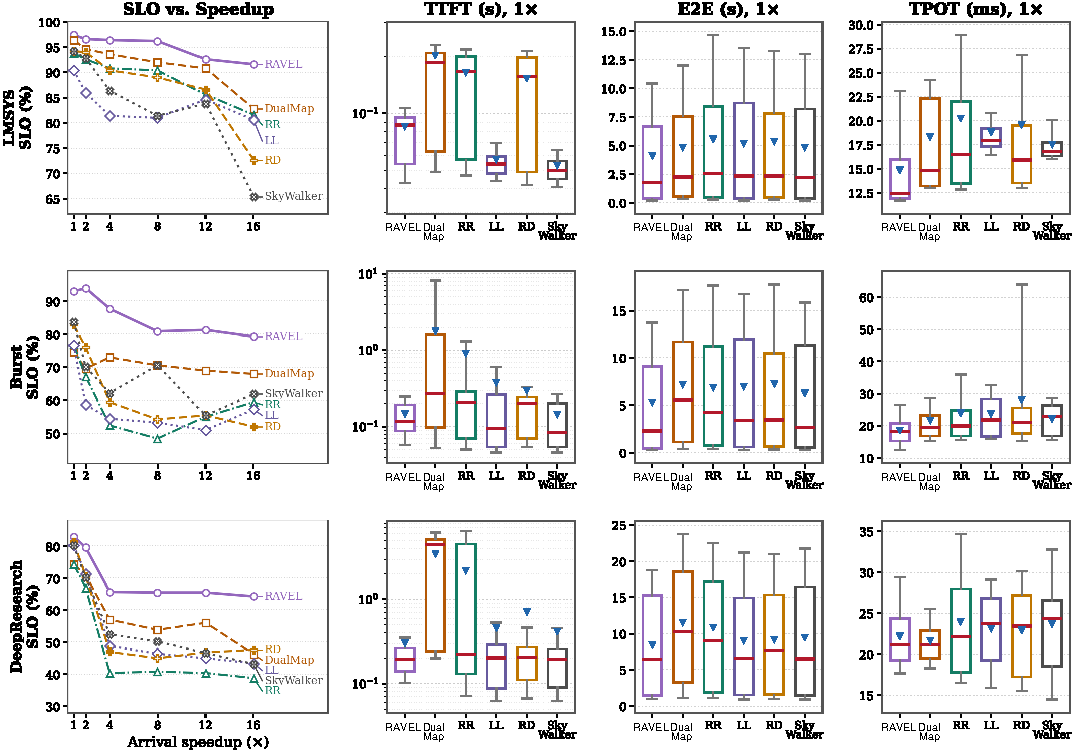
\includegraphics[width=\textwidth]{RAVEL_3DATASETS_4METRICS_ACADEMIC_RAVEL_PURPLE.pdf}
    \caption{
RAVEL preserves higher request-level SLO attainment as offered load increases.
Rows correspond to LMSYS, Burst, and DeepResearch.
The first column varies arrival speedup from $1\times$ to $16\times$; the
remaining columns report TTFT, end-to-end latency, and TPOT distributions at
$1\times$ load.
RAVEL consistently achieves the highest SLO attainment across the evaluated
workloads and loads, without requiring uniformly lower values of every
individual latency metric.
}
    \label{fig:main-results}
\end{figure*}


\section{Evaluation}
\subsection{Experimental Setup}
\label{sec:eval:setup}

\paragraph{Testbed and replay.}
We deploy five Qwen3-1.7B serving replicas across three clusters in a
2/2/1 configuration.  Each replica runs on an NVIDIA GeForce RTX~4090 GPU
with bfloat16 precision using vLLM~0.8.5.post1 (V0).
The final experiments use physical WAN transport rather than synthetic
latency injection; measured directed inter-cluster RTTs range from
10.1 to 37.9\,ms.
Table~\ref{tab:eval-setup} summarizes the common serving configuration.
All policies use the same hardware, topology, and base vLLM configuration;
RAVEL's TBT-aware local control is part of the system evaluated in
Section~\ref{sec:eval:mechanism}.

We replay requests \emph{open-loop}.  For an arrival-rate speedup $s$, we
scale trace inter-arrival times by $1/s$, so control-plane overhead cannot
backpressure the offered load.
We evaluate $1\times$, $2\times$, $4\times$, $8\times$, $12\times$, and
$16\times$ arrival rates, with 500 requests in every
policy--workload--load cell.
Before formal measurement, we warm all backends using the same execution
path.  Before each cell, we reset the prefix cache on every replica,
preventing cached state from carrying across policy comparisons.

\begin{table}[t]
\centering
\small
\caption{Evaluation testbed and serving configuration.}
\label{tab:eval-setup}
\begin{tabular}{@{}ll@{}}
\toprule
\textbf{Dimension} & \textbf{Configuration} \\
\midrule
Model               & Qwen3-1.7B \\
GPU                 & NVIDIA GeForce RTX 4090 \\
Precision           & bfloat16 \\
Serving engine      & vLLM 0.8.5.post1 (V0) \\
Deployment          & 5 replicas / 3 clusters (2/2/1) \\
Network             & Physical WAN \\
Inter-cluster RTT   & 10.1--37.9\,ms (directed) \\
Max. sequences      & 64 per replica \\
Max. batched tokens & 16,384 \\
Prefix caching      & Enabled \\
Chunked Prefill     & Enabled \\
Requests per cell   & 500 \\
Arrival speedup     & $1,2,4,8,12,16\times$ \\
\bottomrule
\end{tabular}
\end{table}

\paragraph{Workloads.}
We evaluate three workload regimes that expose different forms of contention
in geo-distributed serving.
\emph{LMSYS} contains heterogeneous conversational requests with diverse
prompt and response sizes.
\emph{Burst} uses the same 500 request contents as LMSYS but replaces their
arrival timestamps with BurstGPT timestamps.
This controlled construction isolates short-horizon arrival contention from
changes in the request-content distribution.
\emph{DeepResearch} is derived from multi-stage, completion-oriented
workflows.  We flatten branch requests by arrival time and evaluate the first
500 branch requests using request-level completion SLOs; the selected trace
does not define a workflow-level task SLO.
For DeepResearch, RAVEL's semantic output profile is constructed exclusively
from the designated training split and never uses the realized output of an
evaluation request.
Together, the workloads cover heterogeneous conversational traffic,
transient burst contention, and sustained completion-oriented demand.

\paragraph{SLOs.}
We use the JITServe-style heterogeneous-SLO construction implemented by our
evaluation runner.
The base budgets are 0.8\,s for TTFT, 80\,ms for TBT, and 8\,s for
end-to-end completion, with a request-specific multiplier from
$1\times$ to $4\times$.
For LMSYS and Burst, the released class-assignment procedure produces
181 LATENCY, 301 THROUGHPUT, and 18 COLLECTIVE requests in each
500-request trace (seed 42); DeepResearch branch requests are COLLECTIVE.
A LATENCY request succeeds only if its TTFT and every measured TBT satisfy
their respective budgets.
THROUGHPUT and COLLECTIVE requests instead succeed when their end-to-end
latency satisfies the corresponding completion budget.

\paragraph{Baselines.}
We compare RAVEL against five routing policies.
\emph{Round Robin (RR)} is stateless and distributes incoming requests
across serving replicas in round-robin order.
\emph{Least Load (LL)} tracks the number of outstanding requests at each
replica and routes each new request to the replica with the smallest
outstanding-request count.
\emph{Random (RD)} independently selects a serving replica at random for
each incoming request.
\emph{DualMap} jointly considers cache affinity and serving load and
rebalances traffic when affinity-driven placements become hotspots.
\emph{SkyWalker} performs locality-aware cross-region load balancing,
preferring available local capacity and redirecting requests when local
replicas become saturated while preserving prefix locality.
All policies replay identical request records over the same serving topology
and base engine configuration; each baseline uses only the state prescribed
by its routing policy.

\paragraph{Metrics.}
Our primary metric is \emph{request-level SLO attainment}, i.e., the
fraction of requests satisfying the class-specific success criteria above.
We additionally report time to first token (TTFT), time per output token
(TPOT), and end-to-end request latency to separate application-level SLO
outcomes from individual latency components.
For LATENCY requests, we additionally report TBT violations when analyzing
streaming performance.
All evaluated cells complete all 500 requests, and SLO misses remain in the
denominator.




\subsection{End-to-End Performance}
\label{sec:eval:e2e}

Figure~\ref{fig:main-results} summarizes RAVEL's end-to-end performance
across the three workload regimes.
The first column reports request-level SLO attainment as the offered load
increases from $1\times$ to $16\times$.
The remaining columns show the distributions of TTFT, end-to-end latency,
and TPOT at nominal load.
Together, these results characterize RAVEL's SLO attainment under increasing
contention and its latency behavior at nominal load.

\textbf{RAVEL sustains higher SLO attainment under load.}
RAVEL achieves the highest request-level SLO attainment across all three
workloads and every evaluated arrival rate.
The separation is particularly pronounced in several high-contention
settings.
At $16\times$ load, RAVEL attains 91.6\% of request SLOs on LMSYS,
compared with 82.8\% for the best-SLO baseline, DualMap;
79.2\% on Burst, compared with 62.0\% for SkyWalker; and
64.2\% on DeepResearch, compared with 47.6\% for RD.
These correspond to gains of 8.8, 17.2, and 16.6 percentage points,
respectively.
RAVEL therefore retains substantial advantages even when offered load
creates severe contention for serving capacity.

The contrast between LMSYS and Burst provides a controlled view of this
contention.
Burst preserves the same request contents as LMSYS and changes only their
arrival timestamps.
RAVEL's larger advantage on Burst therefore coincides with greater
short-horizon arrival contention rather than a change in the prompt or
response distribution.
The DeepResearch results further show that RAVEL's gains extend beyond mixed
interactive traffic to sustained completion-oriented demand.

\textbf{RAVEL improves SLO attainment while maintaining competitive
latency.}
At nominal load, RAVEL's TTFT, end-to-end latency, and TPOT distributions
remain competitive with the baselines across all three workloads.
Its SLO gains under stress are also accompanied by favorable P95 latency.
At $16\times$ load, RAVEL achieves both higher request-level SLO attainment
and lower P95 TTFT and P95 end-to-end latency than the best-SLO baseline for
each workload.
For example, on Burst, RAVEL reduces P95 TTFT from 8.70\,s to 2.68\,s and
P95 end-to-end latency from 28.68\,s to 18.78\,s relative to SkyWalker,
while increasing SLO attainment from 62.0\% to 79.2\%.
These results highlight the distinction between optimizing a single latency
statistic and maximizing class-specific request-level SLO attainment.

These end-to-end results establish RAVEL's performance benefit but do not
attribute it to individual mechanisms.
Section~\ref{sec:eval:mechanism} next isolates pre-handoff revisability and
RAVEL's SLO-specific execution controls.

\begin{figure*}[t]
    \centering
    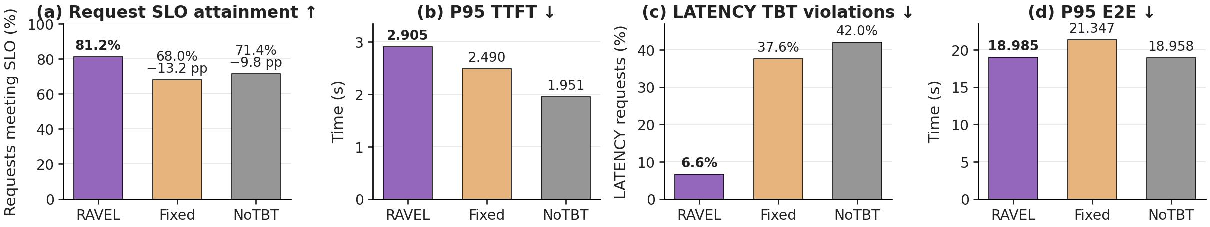
\includegraphics[width=\textwidth]{fig3_mechanism_breakdown.pdf}
    \caption{
\textbf{Mechanism breakdown on Burst at $12\times$ load.}
\emph{FixedPlacement} retains immediate demand accounting but disables
pre-handoff reassignment; \emph{NoTBTGuard} retains Router-side RAVEL
placement but disables the local TBT-aware Chunked-Prefill guard.
We report (a) request-level SLO attainment, (b) P95 TTFT,
(c) the fraction of LATENCY requests with at least one TBT violation, and
(d) P95 end-to-end latency.
Both pre-handoff revisability and local TBT protection materially contribute
to RAVEL's SLO gains.
}
    \label{fig:mechanism-breakdown}
\end{figure*}
\subsection{Mechanism Breakdown}
\label{sec:eval:mechanism}

We next isolate the mechanisms behind RAVEL's end-to-end gains using the
Burst workload at $12\times$ load, where short-horizon contention is strong
while the request contents remain identical to LMSYS.
Figure~\ref{fig:mechanism-breakdown} compares full RAVEL with two ablations:
\emph{FixedPlacement}, which preserves immediate prospective demand
accounting but prevents a tentative replica assignment from changing before
engine handoff, and \emph{NoTBTGuard}, which preserves the global RAVEL
routing policy but disables the local TBT-aware Chunked-Prefill guard.
Each variant processes the same 500-request trace.
The TBT-violation metric is computed over the 181 LATENCY requests in that
trace.

\textbf{Pre-handoff revisability materially improves SLO attainment.}
Freezing the initial tentative placement reduces request-level SLO attainment
from 81.2\% to 68.0\%, a 13.2 percentage-point drop
(Figure~\ref{fig:mechanism-breakdown}a).
Importantly, FixedPlacement still accounts arrived demand immediately, so
later requests observe the load created by earlier tentative assignments.
What it removes is the ability to act on newly revealed demand by revising
those earlier assignments.
The resulting degradation therefore shows that demand visibility alone is
insufficient: earlier placements must remain revisable while they are still
under Router control.
This effect is also visible in streaming performance, where the LATENCY TBT
violation rate increases from 6.6\% under RAVEL to 37.6\% under
FixedPlacement (Figure~\ref{fig:mechanism-breakdown}c).

The result is particularly notable because FixedPlacement does not have worse
TTFT.
Its P95 TTFT is 2.49\,s, compared with 2.91\,s for RAVEL
(Figure~\ref{fig:mechanism-breakdown}b), yet it satisfies substantially fewer
complete request SLOs.
This reinforces the distinction between optimizing one latency component and
preserving the joint SLO constraints that determine whether a request
actually succeeds.

\textbf{Global placement and local TBT protection address complementary
sources of SLO loss.}
Disabling RAVEL's local TBT guard lowers request-level SLO attainment from
81.2\% to 71.4\%, a 9.8 percentage-point reduction.
The clearest change is in the LATENCY requests: their TBT violation rate rises
from 6.6\% to 42.0\%.
At the same time, NoTBTGuard has a lower P95 TTFT than RAVEL
(1.95\,s versus 2.91\,s) and nearly identical P95 end-to-end latency
(18.96\,s versus 18.99\,s).
The degradation is therefore concentrated in the streaming constraint that
the guard is designed to protect rather than in a broad increase in
completion latency.
These results show that selecting an appropriate replica globally is not
sufficient by itself; the local serving path must also bound Prefill
interference in accordance with activ e TBT requirements.

Together with the LateBind experiment in Figure~\ref{fig:motivation}, these
ablations separate the two parts of RAVEL's core design.
Late binding delays commitment but also delays regional demand attribution,
whereas FixedPlacement makes demand visible immediately but removes
pre-handoff revisability.
RAVEL combines both properties: arrived demand influences subsequent
placement decisions immediately, while tentative assignments remain
changeable until engine handoff.


\begin{figure}[t]
    \centering
    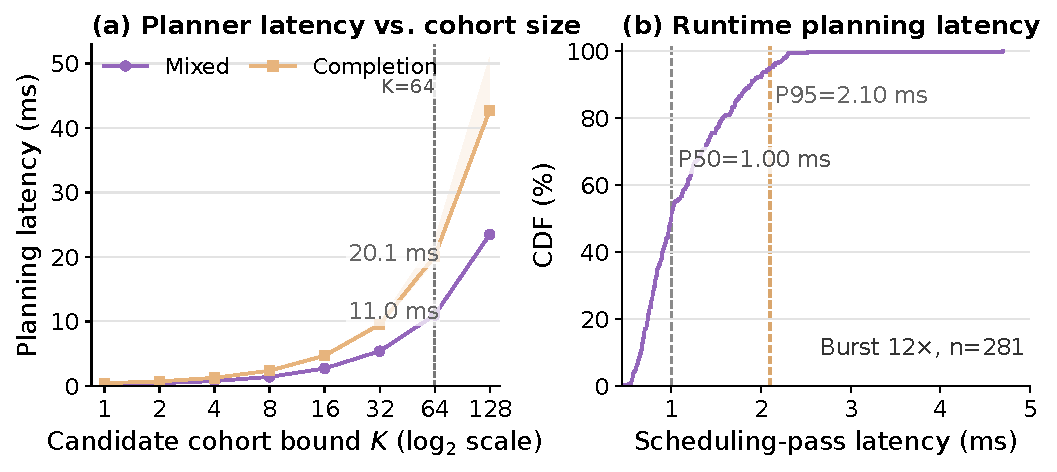
\includegraphics[width=\columnwidth]{fig4_planner_overhead.pdf}
    \caption{
    \textbf{RAVEL control-plane scalability and runtime overhead.}
    (a) Planner latency versus candidate-cohort size for the mixed-traffic
    WorkYield and completion OnTimeSet planners; the dashed line marks the
    mixed-path bound $K=64$.
    (b) CDF of scheduling-pass latency in a 500-request Burst run at
    $12\times$ load.
    The runtime median/P95 are 1.00/2.10\,ms, while the mean/P95 candidate
    cohort sizes are 3.65/7 requests.
    }
    \label{fig:planner-overhead}
\end{figure}

\subsection{Control-Plane Scalability and Overhead}
\label{sec:eval:overhead}

We finally evaluate whether RAVEL's pre-handoff replanning can operate on the
online serving timescale.
Figure~\ref{fig:planner-overhead} separates two questions.
First, we measure how planner latency scales with the size of the candidate
cohort using states derived from the Burst and DeepResearch traces.
For each planner and cohort size, we run five warm-up iterations followed by
50 measured repetitions on an isolated CPU.
Second, we instrument an end-to-end Burst run at $12\times$ load and report
the distribution of planning latency observed during actual execution.

\textbf{Bounded replanning keeps multi-request planning tractable.}
Figure~\ref{fig:planner-overhead}a varies the candidate cohort from 1 to
128 requests for both RAVEL planning paths.
Planning cost increases with cohort size, with the completion planner
consistently more expensive because it additionally considers protected-set
replacement and deferred-request retries.
At RAVEL's normal cohort bound of $K=64$, the median planning latency is
10.99\,ms for the mixed planner and 20.10\,ms for the completion planner;
their P95 latencies are 11.18\,ms and 22.61\,ms, respectively.
Even when the replayed cohort is increased to 128 requests, median latency
remains 23.47\,ms for mixed traffic and 42.75\,ms for completion traffic.
These measurements show the role of the cohort bound: RAVEL does not require
multi-request optimization over the entire Router-owned queue, but confines
the more expensive placement computation to an explicitly bounded working
set.

\textbf{Online planning usually operates far below the configured bound.}
Figure~\ref{fig:planner-overhead}b reports all 281 planning passes from a
500-request Burst run at $12\times$ load.
The median planning latency is 1.00\,ms, with P95 and P99 latencies of
2.10\,ms and 2.30\,ms, respectively; the maximum observed pass takes
4.70\,ms.
The reason actual costs are substantially below the $K=64$ replay point is
that online cohorts are typically small: the mean cohort size is 3.65,
the P95 is 7, and the maximum observed cohort is 9.
Thus, the configured bound protects the control plane against unusually
large reversible sets, while the common online path replans only a small
number of requests at a time.

Overall, these results show that preserving pre-handoff placement
revisability does not require continuously solving a large global assignment
problem.
RAVEL instead performs bounded multi-request replanning when additional
information becomes available, and the measured online planning path remains
at millisecond-scale latency under the evaluated burst workload.



\section{Related Work}
\label{sec:related}

\paragraph{Distributed and geo-distributed LLM routing.}
Distributed LLM serving systems increasingly incorporate runtime load and
cache locality into request routing.
Preble jointly considers reusable KV state and computation load when
scheduling prompts across distributed replicas~\cite{preble}, while DualMap
balances cache affinity against load and performs hotspot-aware
rebalancing~\cite{dualmap}.
Recent systems explicitly target geographically distributed serving.
SkyWalker handles cross-region traffic while preserving KV-cache locality and
load balance~\cite{skylb};
GORGO incorporates WAN latency, queueing state, and Prefill/cache cost into
cross-region routing decisions~\cite{gorgo};
and recent work such as Solyx combines serving telemetry with WAN
measurements for per-request cross-site placement~\cite{solyx}.
Although these systems may redirect or rebalance traffic after an initial
choice, RAVEL differs in the control abstraction it exposes:
it explicitly couples \emph{immediate prospective demand accounting} with
\emph{pre-handoff placement revisability}.
An arrived request is accounted at a tentative replica immediately, while
that replica may still change until the request is handed off to the serving
engine.

\paragraph{SLO-aware LLM serving and application scheduling.}
Prior systems also adapt LLM execution to request-level latency and SLO
requirements.
Sarathi-Serve uses Chunked Prefill to reduce Prefill--Decode interference and
control TTFT and inter-token latency~\cite{sarathi}, while DistServe
disaggregates Prefill and Decode and provisions the two phases according to
TTFT and TPOT requirements~\cite{distserve}.
JITServe targets heterogeneous latency-, deadline-, and compound-request
SLOs, scheduling serving capacity from imprecise request information and
refining those estimates as generation progresses~\cite{jitserve}.
AdaServe instead customizes speculative decoding to per-request SLO
requirements~\cite{adaserve}.
Other systems exploit structure across related LLM calls:
Parrot exposes application-level semantic dependencies to coordinate
multi-request execution~\cite{parrot}, and Agentix treats agentic programs as
first-class scheduling entities to optimize program-level end-to-end
latency~\cite{agentix}.
Libra further partitions requests into cooperating micro-requests and combines
global split-point decisions with local SLO-aware batching to balance dynamic
serving load across instances~\cite{libra}.
RAVEL applies the same broad principle of request-specific SLO awareness at a
different control layer: it uses WAN delay and replica serving state to
determine which geographic capacity remains viable for each request before
engine handoff.
Its local Prefill control complements this global decision by bounding
Prefill interference in accordance with latency-sensitive execution
constraints.

\paragraph{Dynamic reassignment and migration.}
Serving systems can also revise placement after an initial assignment.
Llumnix dynamically reschedules requests across model instances and uses live
migration to improve load balancing and isolation, mitigate resource
fragmentation, and differentiate request priorities and SLOs~\cite{llumnix}.
Such migration preserves placement flexibility even after execution state has
materialized.
RAVEL chooses an earlier control boundary: a request remains reassignable
while it is Router-owned, but its placement becomes final after successful
engine handoff.
Thus, RAVEL performs reassignment before changing placement would require
coordination with engine-managed request state, whereas migration systems
retain flexibility after that state already exists.
The two approaches are complementary: pre-handoff replanning can avoid some
state movement, while runtime migration can correct imbalance that emerges
after execution begins.



\section{Conclusion}

Geo-distributed LLM serving must route requests online even though regional
capacity is request-dependent: a region that is interchangeable for one
request may be essential for satisfying another request's SLO.
Later arrivals can reveal this opportunity cost, but waiting for such
information consumes the same requests' SLO slack.
RAVEL addresses this tension by separating demand visibility from placement
commitment.
It accounts each request immediately at a tentative replica, while keeping
that placement revisable as long as the request remains Router-owned and
committing it only at successful engine handoff.
Across LMSYS, bursty traffic, and multi-stage DeepResearch workloads, RAVEL
consistently improves request-level SLO attainment while maintaining
competitive latency, with particularly large gains under several
high-contention settings.
More broadly, RAVEL shows that an online serving system need not postpone
demand accounting to preserve the flexibility to exploit information revealed
by later arrivals.





{\footnotesize \bibliographystyle{acm}
\bibliography{sample}}


\theendnotes

\end{document}







